\section{ARQUITETURA DE SOFTWARE E TECNOLOGIAS}

As decisões de arquitetura organizam a solução de software e orientam o detalhamento de seus componentes. Pressman e Maxim (2021) tratam o projeto arquitetural como uma etapa própria do processo de projeto, anterior ao projeto em nível de componentes. Para apoiar a comunicação dessas decisões, a ISO/IEC/IEEE 42010:2022 estabelece requisitos para estruturar e expressar descrições de arquitetura, incluindo pontos de vista e modelos, e distingue a arquitetura da descrição que a representa (ISO/IEC/IEEE, 2022).

Essa perspectiva permite apresentar não apenas quais tecnologias foram escolhidas, mas também como os elementos implementados se distribuem e se relacionam, sem confundir as capacidades oferecidas pelos provedores com funcionalidades verificadas no aplicativo. Assim, o capítulo começa pela arquitetura e pelas tecnologias da aplicação móvel; em seguida, descreve os serviços em nuvem, os mecanismos de segurança e a integração de mensageria; por fim, aborda a persistência e o ciclo de vida das publicações, além da lógica de correspondência automatizada entre anúncios.

\subsection{Arquitetura e tecnologias da plataforma}

Para situar os componentes e as integrações utilizados na aplicação, a Figura~\ref{fig:arquitetura_wefind} apresenta uma visão geral da arquitetura do WeFIND.

\begin{figure}[H]
    \centering
    \caption{Arquitetura da plataforma WeFIND}
    \label{fig:arquitetura_wefind}
    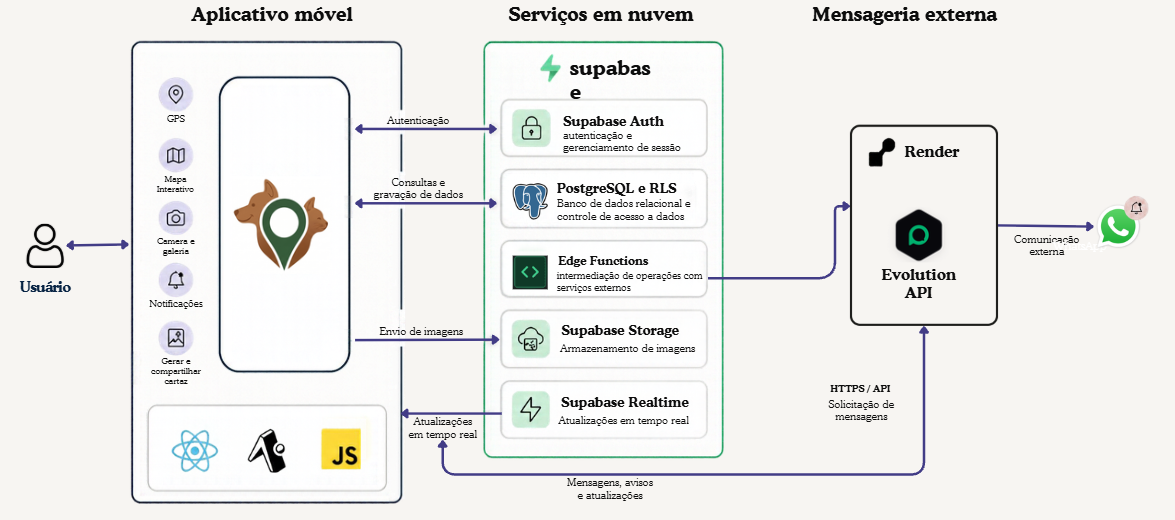
\includegraphics[width=\textwidth]{imagens/03_arquitetura_design/figura13_arquitetura_wefind.png}
    \fonte{Autoria própria (2026), com auxílio de ferramenta de inteligência artificial}
\end{figure}

A Figura~\ref{fig:arquitetura_wefind} apresenta três componentes: o cliente móvel, os serviços de backend do Supabase e o provedor externo de mensageria. O aplicativo concentra a interface e os recursos do dispositivo; o Supabase oferece autenticação, banco de dados, armazenamento e atualização em tempo real; e a Evolution API, hospedada no Render, intermedeia o envio de mensagens pelo WhatsApp.

A aplicação móvel foi desenvolvida com React Native, React e Expo. A Figura~\ref{fig:principais_tecnologias} destaca as principais tecnologias adotadas no projeto.

\begin{figure}[H]
    \centering
    \caption{Principais tecnologias que compõem a plataforma WeFIND}
    \label{fig:principais_tecnologias}
    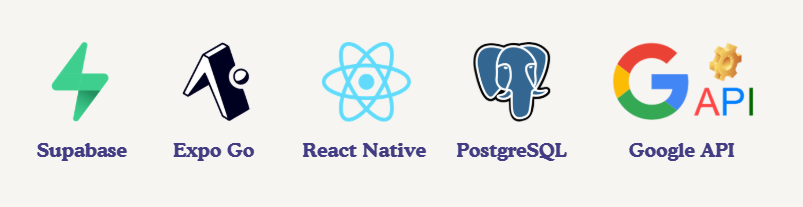
\includegraphics[width=0.82\textwidth]{imagens/03_arquitetura_design/figura11_principais_tecnologias.png}
    \fonte{Autoria própria (2026)}
\end{figure}

A biblioteca React Native foi adotada como núcleo para a interface móvel, em integração com o React. Foram utilizados React Native 0.81.5, React 19.1.0 e Expo SDK 54 (pacote \textit{expo} 54.0.29). O código da aplicação foi desenvolvido em JavaScript com JSX (React, 2026; React Native, 2026; Expo, 2026).

Em relação ao desenvolvimento puramente nativo (como construir separadamente uma aplicação em Kotlin para Android e outra em Swift para iOS), a abordagem isolada exigiria a manutenção de duas bases de código distintas. Para este projeto individual, o React Native permitiu desenvolver para as plataformas móveis a partir de uma base de código compartilhada em JavaScript e JSX.

Em relação a soluções baseadas em \textit{WebView}, o React Native permite compor a interface com componentes nativos e integrar recursos do dispositivo por meio de módulos. Não foi realizado um benchmark comparativo de desempenho entre essas abordagens no projeto.

Em conjunto com o React Native, utilizou-se a plataforma Expo e seus módulos: \textit{expo-location} 19.0.8 para consultar os serviços de localização disponíveis no dispositivo; \textit{expo-image-picker} 17.0.10 para acesso à câmera e à galeria; e \textit{expo-image-manipulator} 14.0.8 para comprimir fotos antes do envio. A precisão das coordenadas depende do aparelho, das permissões concedidas e das condições de recepção (Expo, 2026).

A camada cartográfica baseia-se em \textit{react-native-maps} 1.20.1, responsável pela renderização dos mapas do Google Maps e Apple Maps e pela exibição de marcadores. Para gerar os cartazes com código QR, empregou-se \textit{react-native-view-shot} 4.0.3, que captura a interface como imagem, junto ao módulo \textit{expo-sharing} 14.0.8 para abrir o compartilhamento nativo. A navegação entre telas utiliza \textit{@react-navigation/native} 7.1.25. A estilização visual adotou NativeWind 4.2.1, baseado em Tailwind CSS 3.4.19 (React Native Maps, 2026; React Native View Shot, 2026; Expo, 2026; React Navigation, 2026; NativeWind, 2026; Tailwind CSS, 2026).

No Android, a visualização cartográfica utiliza o provedor Google Maps por meio da configuração da chave da Google Maps Platform, enquanto a biblioteca \textit{react-native-maps} integra o mapa à interface. A aplicação também pode abrir o Google Maps por meio de uma URL externa para apresentar a localização de uma publicação ou orientar o usuário até o ponto indicado. O funcionamento depende da conexão, das permissões de localização e da configuração válida da chave (Google Maps Platform, 2026; React Native Maps, 2026).

Os formulários também validam campos obrigatórios, verificam a sintaxe de endereços de e-mail e formatam números telefônicos antes do envio. Essas verificações no cliente apoiam a validação de entrada, mas não substituem os controles aplicados nos serviços de backend.

Para apoiar o desenvolvimento, utilizaram-se Node.js, npm e Visual Studio Code na implementação; Git e GitHub no controle de versões; Trello na organização das tarefas com Kanban; Astah UML na modelagem; e Figma na prototipação. ChatGPT e GitHub Copilot foram empregados como ferramentas auxiliares de programação e produção de conteúdo (OpenAI, 2026; GitHub, 2026). A Figura~\ref{fig:ferramentas_auxiliares} reúne parte desses recursos.

\begin{figure}[H]
    \centering
    \caption{Ferramentas auxiliares de apoio ao desenvolvimento do projeto}
    \label{fig:ferramentas_auxiliares}
    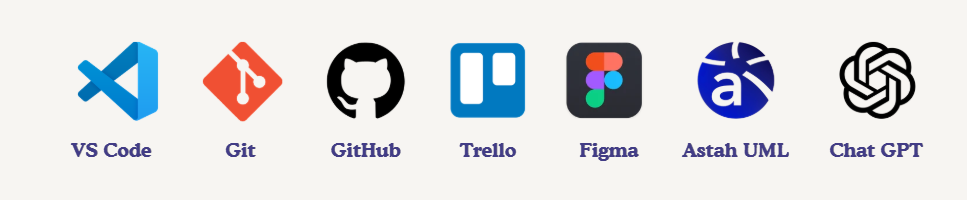
\includegraphics[width=0.88\textwidth]{imagens/03_arquitetura_design/figura12_ferramentas_auxiliares.png}
    \fonte{Autoria própria (2026)}
\end{figure}

\subsection{Serviços em nuvem, segurança e mensageria}

O backend utiliza a plataforma Supabase (Supabase, 2026) e a biblioteca cliente \textit{@supabase/supabase-js} 2.87.3. O Supabase reúne os serviços de autenticação, banco de dados PostgreSQL, armazenamento de arquivos e atualização em tempo real empregados pelo aplicativo; a versão dos serviços gerenciados é administrada pela plataforma. Essa composição foi escolhida para atender às necessidades do projeto sem desenvolver e manter todos esses componentes separadamente.

O Supabase Auth também intermedeia a autenticação social com o Google. Nesse fluxo, o aplicativo solicita ao Supabase uma URL de autenticação, abre o navegador do dispositivo para que o usuário conclua o login na conta Google e, após o retorno por um esquema de redirecionamento próprio do aplicativo, troca o código recebido por uma sessão autenticada. Dessa forma, o WeFIND não coleta nem armazena a senha da conta Google; a autenticação é realizada pelo provedor externo e a sessão resultante é gerenciada pelo Supabase Auth (Supabase, 2026).

Para este projeto, o PostgreSQL foi selecionado por oferecer um modelo relacional adequado às relações entre perfis, publicações, imagens, avistamentos e conversas. Essa escolha descreve a necessidade atendida pelo WeFIND e não implica que bancos NoSQL sejam inadequados para outros sistemas.

O Supabase também foi preferido a implementar e operar, no escopo do projeto, serviços próprios para autenticação, persistência e armazenamento. Essa decisão reduz a quantidade de infraestrutura que a equipe precisa administrar diretamente, mas não elimina a dependência das configurações e da disponibilidade do provedor.

No login com o Google, o aplicativo utiliza o fluxo OAuth com PKCE e delega a autenticação ao Supabase Auth; a senha da conta Google não é coletada pelo aplicativo. As políticas de segurança em nível de linha (RLS) são configuradas no banco, com regras específicas para cada tabela. No esquema consultado, a leitura anônima de dados de perfis, publicações e avistamentos foi restringida; as regras de avistamentos e conversas também limitam o acesso conforme autenticação e participação. Assim, o comportamento de acesso depende das políticas efetivamente configuradas para cada entidade, não de uma garantia uniforme para todo o banco.

As funções de borda concentram operações que usam credenciais de provedores externos. A chave da Evolution API é mantida como variável de ambiente no servidor, fora do aplicativo móvel; a função de mensageria exige uma sessão autenticada para receber solicitações de envio.

Os códigos temporários de cadastro, recuperação de senha e alteração de telefone são representados no armazenamento por resumos SHA-256, possuem prazo de validade e são removidos após o uso. O fluxo limita as tentativas de validação e aplica intervalo mínimo entre novas solicitações. Os registros de log também foram ajustados para evitar a exposição de credenciais e dados sensíveis.

Backups, restauração, expiração global de sessões e disponibilidade dependem das configurações e dos serviços dos provedores Supabase e Render; não são garantias fornecidas exclusivamente pelo aplicativo.

Para a comunicação com o WhatsApp, utilizou-se a Evolution API (Evolution API, 2026), hospedada no Render (Render, 2026). No ambiente utilizado, a integração por requisições HTTP REST apoiou o envio de códigos de recuperação de senha e de avisos de avistamento. A disponibilidade e eventuais custos da hospedagem e dos serviços externos dependem dos respectivos provedores.

\subsection{Persistência e ciclo de vida das publicações}

A persistência estruturada utiliza o PostgreSQL. A Figura~\ref{fig:modelo_logico_banco} apresenta o modelo lógico relacional adotado no projeto e os relacionamentos entre as entidades representadas.

\begin{figure}[H]
    \centering
    \caption{Modelo Lógico Relacional do Banco de Dados PostgreSQL}
    \label{fig:modelo_logico_banco}
    \includegraphics[width=0.95\textwidth]{imagens/02_modelagem/figura09_modelo_logico_banco.png}
    \fonte{Autoria própria (2026)}
\end{figure}

Na Figura~\ref{fig:modelo_logico_banco}, os nomes representados são \textit{usuarios}, \textit{animais}, \textit{publicacoes}, \textit{fotos\_publicacoes}, \textit{avistamentos} e \textit{mensagens}. A seguir, descreve-se o conteúdo dessas entidades conforme o modelo apresentado na figura.

A entidade \textit{usuarios} centraliza os dados cadastrais dos participantes do sistema. Seu identificador primário conecta-se à chave única fornecida pelo serviço Supabase Auth e relaciona informações como nome, endereço de e-mail, fotografia de perfil, telefone, cidade, estado e data de criação da conta.

A entidade \textit{animais} representa os animais domésticos associados aos usuários no modelo apresentado.

A entidade \textit{publicacoes} reúne anúncios georreferenciados de animais perdidos ou encontrados. Cada registro relaciona-se ao usuário responsável e, no modelo, pode referenciar um animal cadastrado. Também contempla título, descrição, coordenadas, endereço, data do fato, situação de resolução, datas de criação e atualização e prazo de expiração.

A entidade \textit{fotos\_publicacoes} organiza as imagens associadas às publicações, mantendo uma relação de um para muitos com \textit{publicacoes} e registrando o endereço dos arquivos armazenados.

A entidade \textit{avistamentos} reúne relatos da comunidade sobre animais observados em outros locais ou momentos. Cada registro associa-se à publicação e ao usuário informante e pode incluir localização, descrição, fotografia e data do relato.

A entidade \textit{mensagens} representa a comunicação entre participantes, relacionando a publicação em discussão, remetente, destinatário, conteúdo, eventual anexo, estado de leitura e data de envio.

O modelo também prevê estruturas de apoio à comunicação de avisos e à moderação, relacionadas aos requisitos de notificações e denúncias.

As publicações têm vigência ativa de 30 dias, contados a partir do cadastro ou da última renovação. Três dias antes do vencimento, o aplicativo pode enviar um aviso para que o responsável renove o anúncio. Sem renovação, a publicação fica inativa e deixa de aparecer no mural e no mapa público, mas ainda pode ser renovada durante o período adicional de 30 dias.

Após o período de carência, a publicação pode ser removida permanentemente pela rotina de limpeza acionada durante o carregamento do mural, com intervalo mínimo de uma hora entre verificações na mesma execução do aplicativo. No fluxo de limpeza local, são considerados somente os anúncios do usuário autenticado, e a exclusão também remove os registros das fotos relacionadas e os arquivos correspondentes no Supabase Storage. Portanto, o sistema não executa uma varredura global: a remoção definitiva das publicações de cada conta depende da execução da rotina no contexto dessa conta.

\subsection{Correspondência automatizada entre publicações}

O WeFIND compara publicações não resolvidas de animais perdidos e encontrados para sugerir possíveis correspondências. Antes de calcular a pontuação, a rotina descarta pares com espécies incompatíveis, sexo informado como oposto ou porte classificado nos extremos pequeno e grande/gigante. Para os demais pares, soma bônus e penalidades definidos para atributos do animal e proximidade geográfica, calculada pela fórmula de Haversine quando há coordenadas. O resultado é um índice heurístico entre 0 e 100, limitado nessa faixa e arredondado; não representa uma probabilidade estatística de reencontro. O \hyperlink{quadro:matching}{Quadro~4} resume as regras implementadas.

\vspace{0.3cm}
{
\phantomsection\hypertarget{quadro:matching}{}
\small
\renewcommand{\arraystretch}{1.12}
\begin{longtable}{|>{\raggedright\arraybackslash}p{3.3cm}|>{\raggedright\arraybackslash}p{8.4cm}|>{\centering\arraybackslash}p{2.5cm}|}
\hline
\multicolumn{3}{|c|}{\textbf{Quadro 4: Critérios e Pesos do Algoritmo de Correspondência do WeFIND}} \\ \hline
\label{quadro:matching}
\textbf{Critério Avaliado} & \textbf{Condição Lógica e Regra de Negócio} & \textbf{Pontuação} \\ \hline
\endfirsthead

\hline
\multicolumn{3}{|c|}{\textbf{Quadro 4: Critérios e Pesos do Algoritmo de Correspondência (Continuação)}} \\ \hline
\textbf{Critério Avaliado} & \textbf{Condição Lógica e Regra de Negócio} & \textbf{Pontuação} \\ \hline
\endhead

\hline
\multicolumn{3}{|r|}{\textit{Continua na próxima página}} \\ \hline
\endfoot

\hline
\multicolumn{3}{|c|}{\textbf{Fonte:} Autoria própria (2026)} \\ \hline
\endlastfoot

\textbf{Espécie} & Compatível e informada nos dois anúncios. & +20 pontos \\ \cline{2-3}
& Uma das espécies ausente ou genérica. & +10 pontos \\ \cline{2-3}
& Espécies incompatíveis. & Par descartado \\ \hline
\textbf{Sexo} & Mesmo sexo identificado nos dois registros. & +10 pontos \\ \cline{2-3}
& Sexo ausente ou não conclusivo em pelo menos um registro. & +3 pontos \\ \cline{2-3}
& Sexos opostos informados. & Par descartado \\ \hline
\textbf{Porte} & Mesmo porte nos dois anúncios. & +15 pontos \\ \cline{2-3}
& Portes diferentes sem incompatibilidade extrema. & +6 pontos \\ \cline{2-3}
& Porte ausente em um dos registros. & +5 pontos \\ \cline{2-3}
& Porte pequeno/mini comparado a grande/gigante. & Par descartado \\ \hline
\textbf{Raça} & Mesmo texto de raça após normalização. & +25 pontos \\ \cline{2-3}
& Um texto de raça contém o outro após normalização. & +18 pontos \\ \cline{2-3}
& Ambos classificados como SRD, mestiços ou sem raça informada. & +8 pontos \\ \cline{2-3}
& Duas raças informadas e diferentes. & -20 pontos \\ \cline{2-3}
& Um registro classificado como SRD e o outro com raça informada. & +4 pontos \\ \hline
\textbf{Cor da pelagem} & Duas ou mais palavras-chave de cor em comum. & +20 pontos \\ \cline{2-3}
& Uma palavra-chave de cor em comum. & +12 pontos \\ \cline{2-3}
& Cores reconhecidas, sem palavra-chave em comum. & -25 pontos \\ \cline{2-3}
& Cor ausente ou não reconhecida. & +4 pontos \\ \hline
\textbf{Idade} & Mesma idade/faixa textual informada. & +5 pontos \\ \cline{2-3}
& Um filhote comparado a um animal idoso/sênior. & -15 pontos \\ \cline{2-3}
& Demais casos. & Sem pontuação adicional \\ \hline
\textbf{Distância com coordenadas} & Até 1,2~km; até 3,5~km; até 8~km. & +15; +10; +5 pontos \\ \cline{2-3}
& Acima de 8~km até 20~km. & +2 pontos \\ \cline{2-3}
& Acima de 20~km. & -15 pontos \\ \hline
\textbf{Localização sem GPS} & Mesma cidade e mesmo bairro; mesma cidade, sem bairro coincidente. & +12; +5 pontos \\ \cline{2-3}
& Cidades diferentes. & -20 pontos \\ \cline{2-3}
& Sem coordenadas e sem cidade comparável. & Sem pontuação adicional \\ \hline
\end{longtable}
}

O sistema apresenta correspondências com pontuação mínima de 55\% na busca padrão. Já a rotina de notificações aplica o limiar de 60\% e processa até três resultados por publicação. A diferença entre os limites permite exibir sugestões que ainda não acionam notificações automáticas. A pontuação, portanto, serve como critério de ordenação e triagem, não como confirmação de identidade.

O registro de avistamento é um fluxo separado: após a confirmação pelo usuário, o aplicativo grava o relato associado à publicação e atualiza sua localização mais recente, preservando os avistamentos anteriores. A sugestão de correspondência, por si só, não registra um avistamento nem altera a publicação.

Com a definição da arquitetura de software, a modelagem do banco de dados e as ferramentas de desenvolvimento estabelecidas, o Capítulo~7 apresenta o projeto de interface do WeFIND, detalhando os aspectos de usabilidade, a identidade visual e as telas desenvolvidas.
